\clearpage
%%=========================================
\section[Surface Analysis of Substrate B with Surface Pre-Growth Preparation]{Surface Analysis of Substrate B with Surface Pre-Growth Preparation%
   \sectionmark{Surface Analysis of Pre-Growth Substrate B}}\sectionmark{Surface Analysis of Pre-Growth Substrate B}\label{sec:subBb}
   
The dark field images taken of the surface of substrate B after polishing and an etch show that the surface pre-growth preparation has improved the surface considerably, see Fig.~\ref{fig:subBa_om_df} and Fig.~\ref{fig:subBb_om_df}. The previously observed deep surface scratches are removed and there are far less particles on the substrate surface.

\begin{figure}[htbp]
    \centering
    
\includegraphics[width=0.8\linewidth]{subBb_om_n030.jpg}
    \caption[Dark field optical microscopy image of substrate B with surface pre-growth preparation.]{Dark field optical microscopy image of substrate B with surface pre-growth preparation taken in the upper left corner of the substrate at a magnification of $20\times$. The same particle configuration can be observed in both images.}
    \label{fig:subBb_om_df}
\end{figure}
   
   
%%=========================================
   
\begin{figure}[htbp]
    \centering
    
\includegraphics[width=0.8\linewidth]{unknown.png}
    \caption[\Ac{sem} of the centre of substrate B with surface pre-growth preparation.]{\Acf{sem} image taken at the centre of substrate C after surface pre-growth preparation at a  magnification of $5000\times$.}
    \label{fig:subBb_sem_area}
\end{figure}

The surface of substrate B after preparation polish and etch \todo{}. However, there are many tiny particles with lengths of \SIrange{20}{50}{\nano\metre} on the substrate surface. A typical area in the centre of substrate B can be seen in Fig.~\ref{fig:subBb_sem_area}.

The small particles observed in \ac{sem} are distributed evenly over the surface with a tendency of higher density towards the upper right, lower right, and lower left corners. The particle density was found to be between \SI{5e+06}{\particle\centi\metre^{-2}} and \SI{5e+07}{\particle\centi\metre^{-2}}. The mean particle density was \SI{2e+07}{\particle\centi\metre^{-2}} with a standard deviation of \SI{9e+06}{\particle\centi\metre^{-2}}. A graphical representation of the particle density at different locations on substrate C can be seen in Fig.~\ref{fig:subBb_densityData}.

\begin{figure}[htbp]
    \centering
    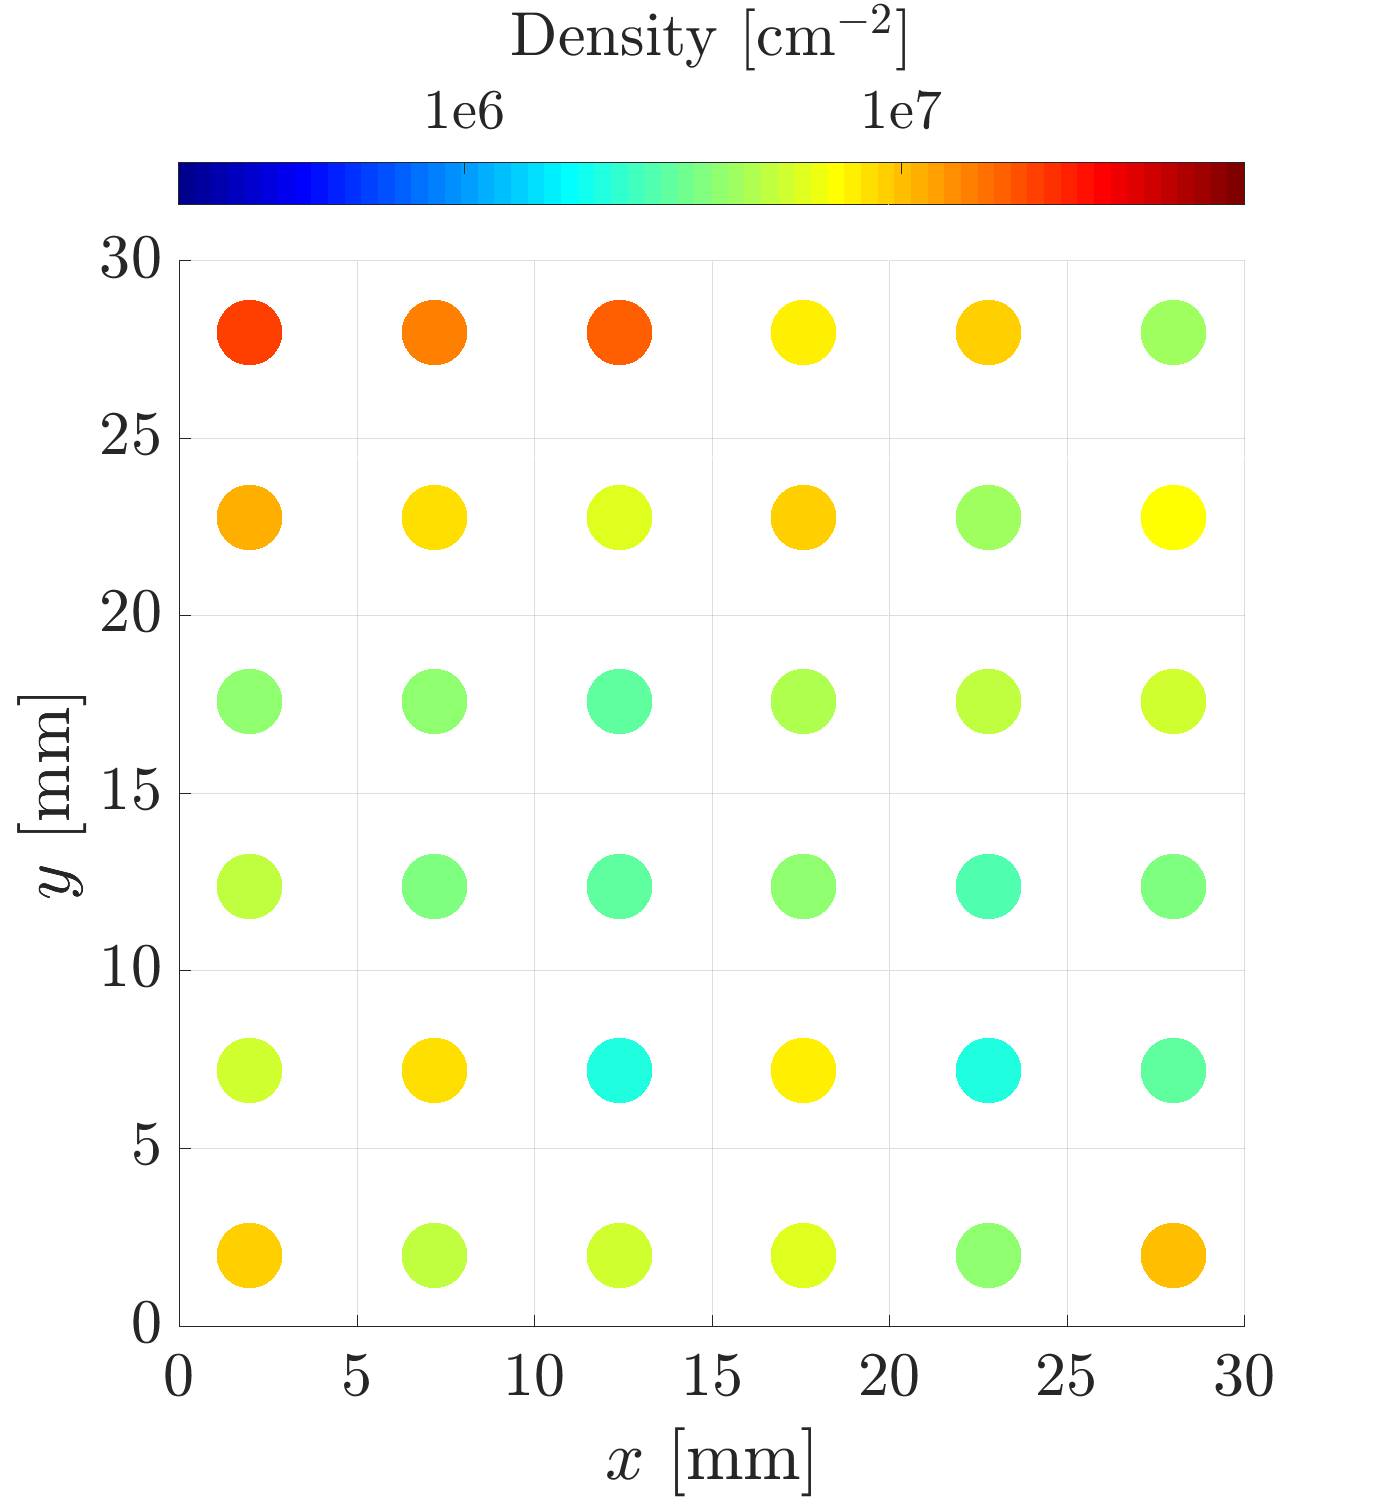
\includegraphics[width=0.8\linewidth]{subBb_densityData.png}
    \caption[Map of the polishing grit density on substrate B after surface pre-growth preparation.]{A map of the polishing grit density at 121 different locations on the $\SI{30}{\milli\metre}\times\SI{30}{\milli\metre}$ substrate B after surface pre-growth preparation. The polishing grit density was observed to vary between \SI{5e+06}{\particle\centi\metre^{-2}} and \SI{5e+07}{\particle\centi\metre^{-2}}.}
    \label{fig:subBb_densityData}
\end{figure}

%%=========================================
\subsection{Particles}
\begin{figure}
    \centering
    \begin{subfigure}[t]{\textwidth}
          \begin{minipage}[t]{0.49\linewidth}
            \centering
            
\includegraphics[width=\linewidth]{unknown.png}
          \end{minipage}
          \hspace{0.02\linewidth}
          \begin{minipage}[t]{0.49\linewidth}
            \centering
            
\includegraphics[width=\linewidth]{unknown.png}
          \end{minipage}
        \caption{\todo{Add caption}}\label{fig:add_label}
    \end{subfigure}
    \par\bigskip
    \begin{subfigure}[t]{\textwidth}
          \begin{minipage}[t]{0.49\linewidth}
            \centering
            
\includegraphics[width=\linewidth]{unknown.png}
          \end{minipage}
          \hspace{0.02\linewidth}
          \begin{minipage}[t]{0.49\linewidth}
            \centering
            
\includegraphics[width=\linewidth]{unknown.png}
          \end{minipage}
        \caption{\todo{Add caption}}\label{fig:add_label}
    \end{subfigure}
    \par\bigskip
    \begin{subfigure}[t]{\textwidth}
          \begin{minipage}[t]{0.49\linewidth}
            \centering
            
\includegraphics[width=\linewidth]{unknown.png}
          \end{minipage}
          \hspace{0.02\linewidth}
          \begin{minipage}[t]{0.49\linewidth}
            \centering
            
\includegraphics[width=\linewidth]{unknown.png}
          \end{minipage}
        \caption{\todo{Add caption}}\label{fig:add_label}
    \end{subfigure}
    \caption[\Ac{sem} images and \ac{eds} spectra of particles found on substrate B after surface pre-growth preparation.]{High resolution \acf{sem} images of particles found on substrate B after surface pre-growth preparation and the corresponding \acf{eds} spectra of the particles.}\label{fig:subBb_sem_w_eds}
\end{figure}

\begin{figure}[htbp]
\ContinuedFloat
    \centering
    \begin{subfigure}[t]{\textwidth}
          \begin{minipage}[t]{0.49\linewidth}
            \centering
            
\includegraphics[width=\linewidth]{unknown.png}
          \end{minipage}
          \hspace{0.02\linewidth}
          \begin{minipage}[t]{0.49\linewidth}
            \centering
            
\includegraphics[width=\linewidth]{unknown.png}
          \end{minipage}
        \caption{\todo{Add caption}}\label{fig:add_label}
    \end{subfigure}
    \captionsetup{list=no}
    \caption{\emph{(continued)}}
\end{figure}


%%=========================================

%%=========================================
%\section{AFM Study of Polished and Etched Substrate B}
\subsection{Surface Roughness}
\begin{figure}[htbp]
    \centering
    \begin{subfigure}[t]{\linewidth}
    \centering
        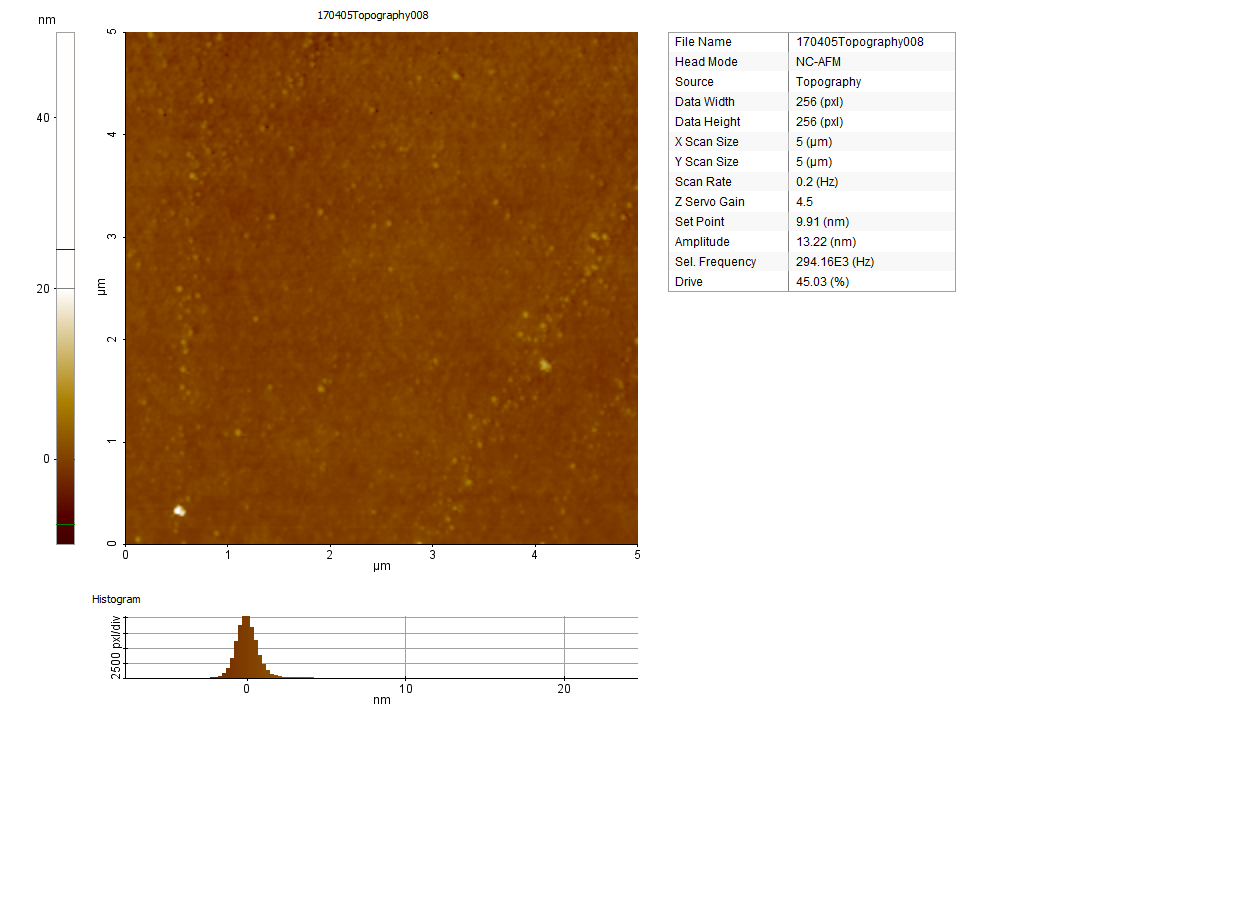
\includegraphics[width=0.5\linewidth,trim={0cm 12cm 21cm 0cm},clip]{170405Topography008_centre.png}
        \caption{Near centre, \ac{rms} roughness \SI{0.85}{\nano\metre}.}%\SI{0.85}{\nano\metre}
    \end{subfigure}%
    \par\bigskip
    \begin{subfigure}[t]{\linewidth}
    \centering
        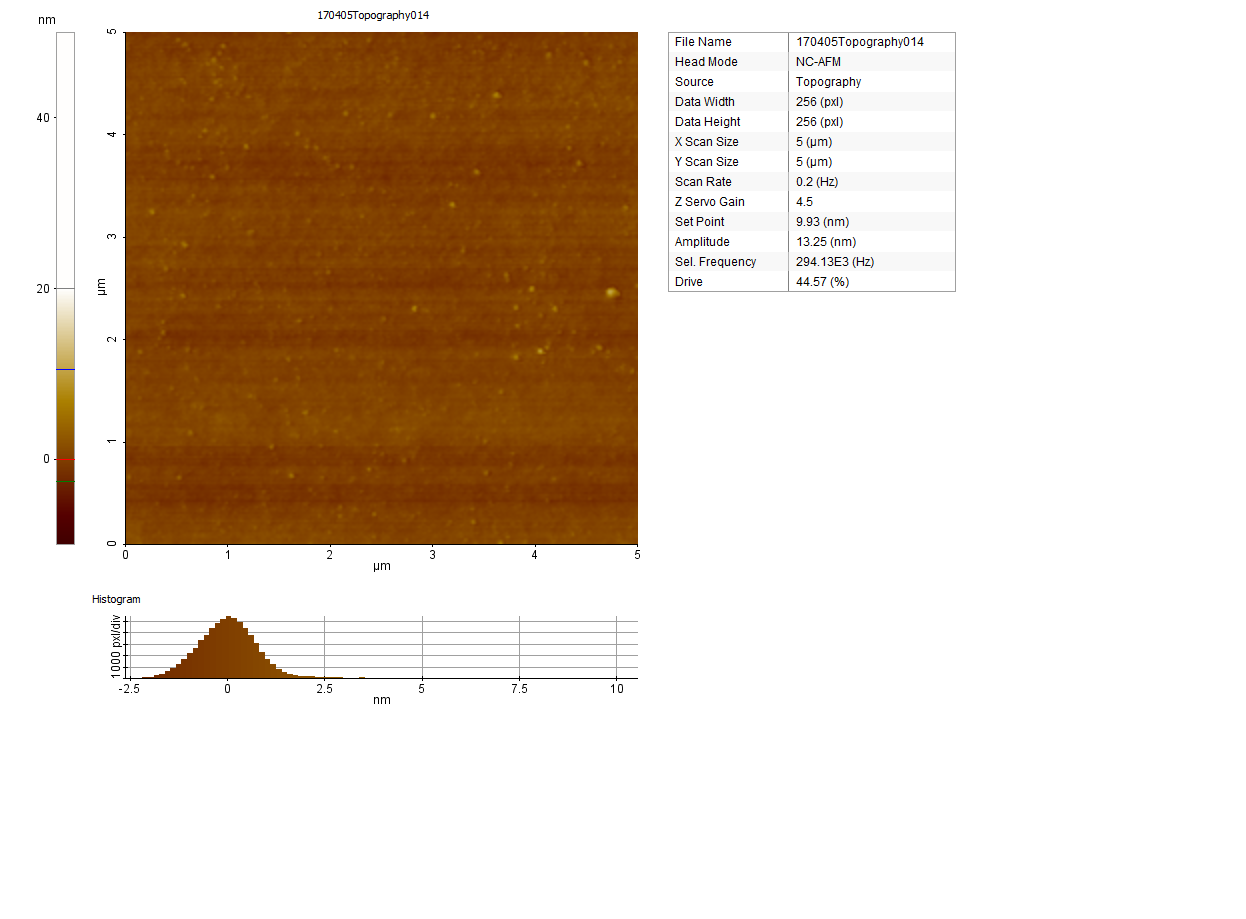
\includegraphics[width=0.5\linewidth,trim={0cm 12cm 21cm 0cm},clip]{170405Topography014_leftedge.png}
        \caption{Near left edge, \ac{rms} roughness \SI{0.76}{\nano\metre}.}%\SI{0.77}{\nano\metre}
    \end{subfigure}%
    \par\bigskip
    \begin{subfigure}[t]{\linewidth}
    \centering
        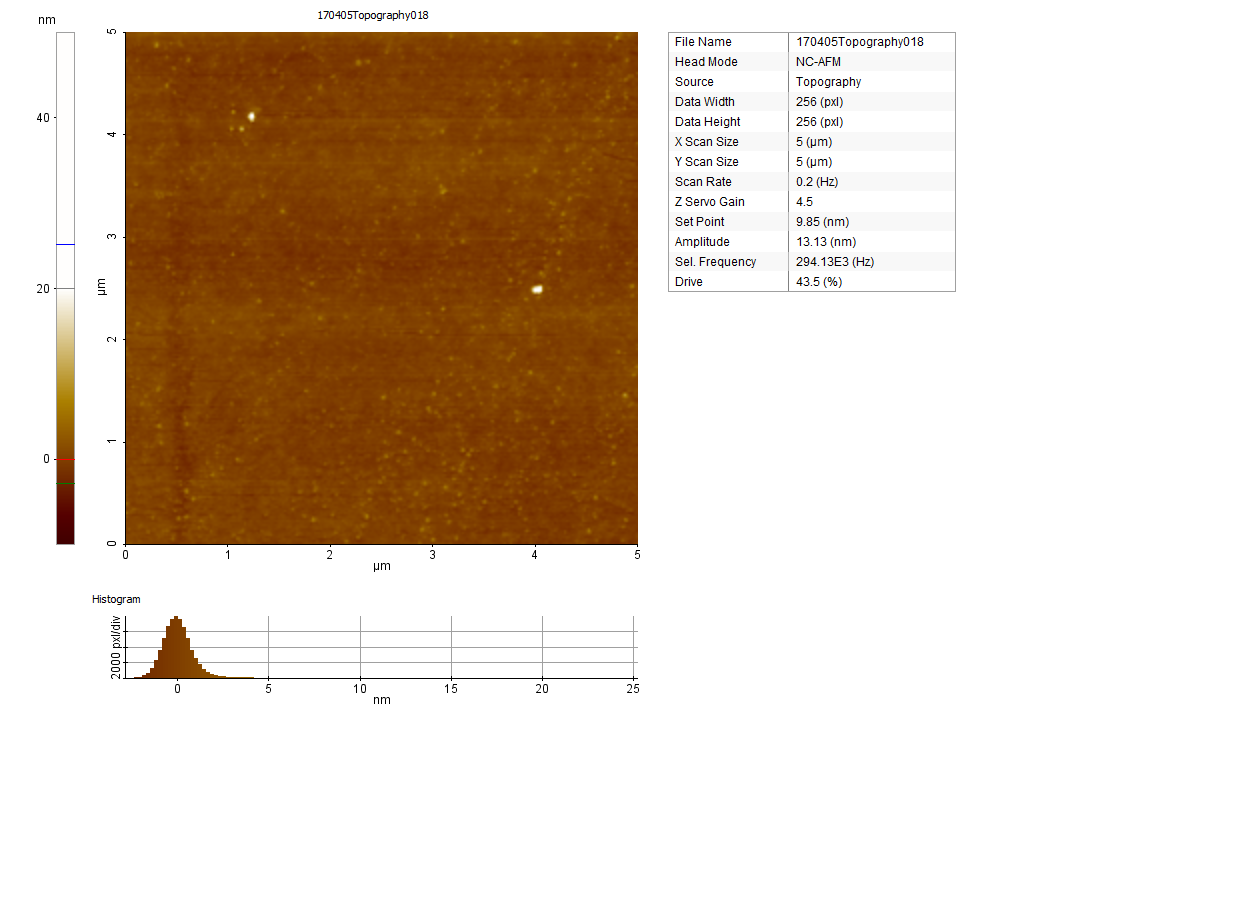
\includegraphics[width=0.5\linewidth,trim={0cm 12cm 21cm 0cm},clip]{170405Topography018_upperleftcorner.png}
        \caption{Near upper left corner, \ac{rms} roughness \SI{0.92}{\nano\metre}.} %\SI{1,04}{\nano\metre}}
    \end{subfigure}%
    \caption[\Ac{afm} of substrate B with surface pre-growth preparation.]{\Acf{afm} measurements of substrate B with surface pre-growth preparation. Images of a $\SI{5}{\micro\metre}\times\SI{5}{\micro\metre}$ area are taken at the centre, edge, and corner of the substrate.}\label{fig:afm_subBb}
\end{figure} % AFM, substrate B, with surface pre-growth preparation.

% B2: AFM: UL - 1.310 nm, U-edge - 0.956, Centre- 0.912 nm

%%=========================================
\subsection{Impurity Analysis}
\begin{table}[htbp]
    \centering
    \caption[\Ac{eds} impurity analysis of substrate B with surface pre-growth preparation.]{Results of the \acf{eds} impurity analysis at three different locations on the $30\times30$ \SI{}{\milli\metre^2} (111)B \ac{czt} substrate B with surface pre-growth preparation (atomic concentration \%). The X-ray signal is acquired from a $\SI{1270}{}\times\SI{890}{\micro\metre^2}$ area centred around the given $X$ and $Y$ values at a magnification of 100$\times$.}\label{tab:subBb_eds_analysis}
    \begin{tabu} to 1.0\textwidth { X[1,c] X[1,c] X[1.125,c] X[1.125,c] X[1.125,c] X[1.125,c] X[1.125,c] X[1.125,c] X[1.125,c] }
    \hline
        \textbf{$X$} (\SI{}{\milli\metre}) &  \textbf{$Y$} (\SI{}{\milli\metre}) & \textbf{\ce{Te}} (at.\%) & \textbf{\ce{Cd}} (at.\%) & \textbf{\ce{Zn}} (at.\%) & \textbf{\ce{Al} } (at.\%) & \textbf{\ce{Si}} (at.\%) & \textbf{\ce{C}} (at.\%) & \textbf{\ce{O}} (at.\%) \\
        \hline
         \SI{1.0}{}  & \SI{29.0}{} & \SI{45.83}{} & \SI{45.34}{} & \SI{1.92}{} & \SI{0.60}{} & \SI{0.50}{} & \SI{5.34}{} & \SI{0.47}{} \\
         \SI{15.0}{} & \SI{29.0}{} & \SI{45.49}{} & \SI{45.12}{} & \SI{2.02}{} & \SI{0.26}{} & \SI{0.49}{} & \SI{5.99}{} & \SI{0.64}{} \\
         \SI{15.0}{} & \SI{15.0}{} & \SI{46.10}{} & \SI{45.35}{} & \SI{1.92}{} & \SI{0.23}{} & \SI{0.52}{} & \SI{5.49}{} & \SI{0.40}{} \\
         \hline
    \end{tabu}
\end{table}
%%=========================================
% FTIR transmission spectra.
\subsection{IR Characterisation}
%%=========================================
